\documentclass[11pt]{article}
%Gummi|061|=)
\title{\textbf{BarChar Report 2.2}}
\author{TianXing He}
\date{}
\usepackage{graphicx}
\usepackage{float}
\begin{document}

\maketitle
%%%%%%%%%%%%%%%%%%%%%%%%%%%%%%%%%%%%%%%%%%%%%%%%%%%%%%%%%%%%%%%%%%%%%%%%%%%%%%%%
\section{BarChart}
To my surprise, the average entropy calculated by the bin and parzen window both expose an ascending nature(I expected it to be descending from the first hidden layer).\\
\textbf{Problem:}There are a lot of 0-bins, I use a htxSmooth method the assign non-zero values to these bins.(by pulling a line from first left bin and first right bin.)
\begin{figure}[H]
\centering
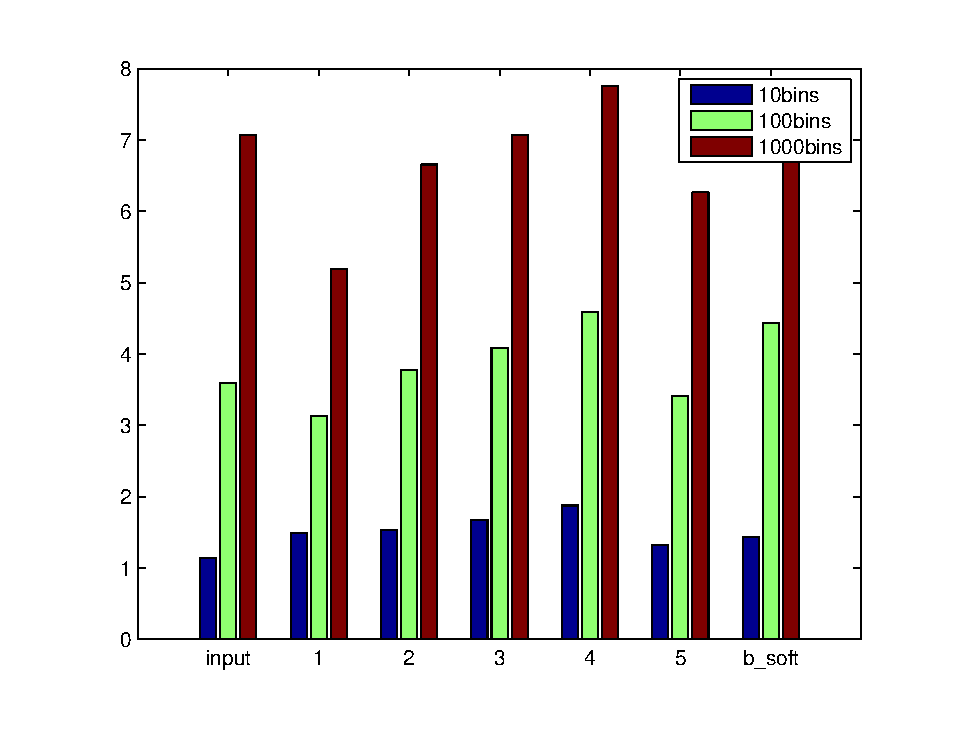
\includegraphics[scale=0.80]{figs/htxSmoothedEntropy.eps}
\caption{entropy after htxSmooth}
\end{figure}
Note that for probability density estimation we assume a continuous distribution, so the entropy is not guaranteed to be greater than zero, I use 1000 sample nodes to calculate the $\int f log2(f) $.
\begin{figure}[H]
\centering
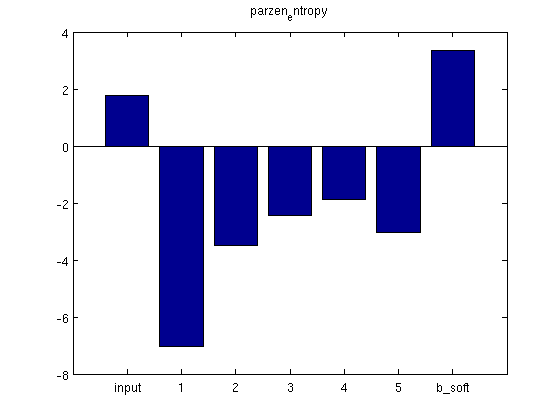
\includegraphics[scale=0.80]{figs/parzen_entropy.png}
\caption{average entropy using parzens}
\end{figure}

%%%%%%%%%%%%%%%%%%%%%%%%%%%%%%%%%%%%%%%%%%%%%%%%%%%%%%%%%%%%%%%%%%%%%%%%%%%%%%%
\section{coefficient}
\begin{figure}[H]
\centering
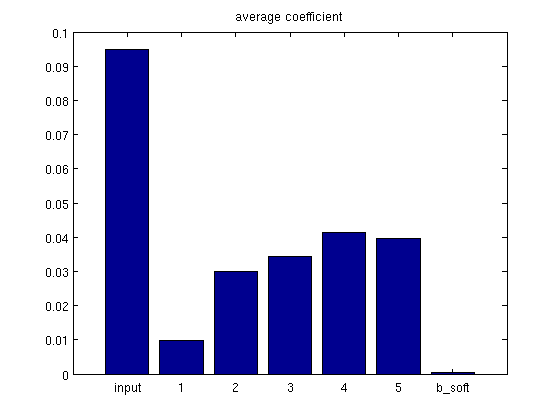
\includegraphics[scale=0.80]{figs/avg_abs_coefficient.png}
\end{figure}
\begin{figure}[htp]
\centering
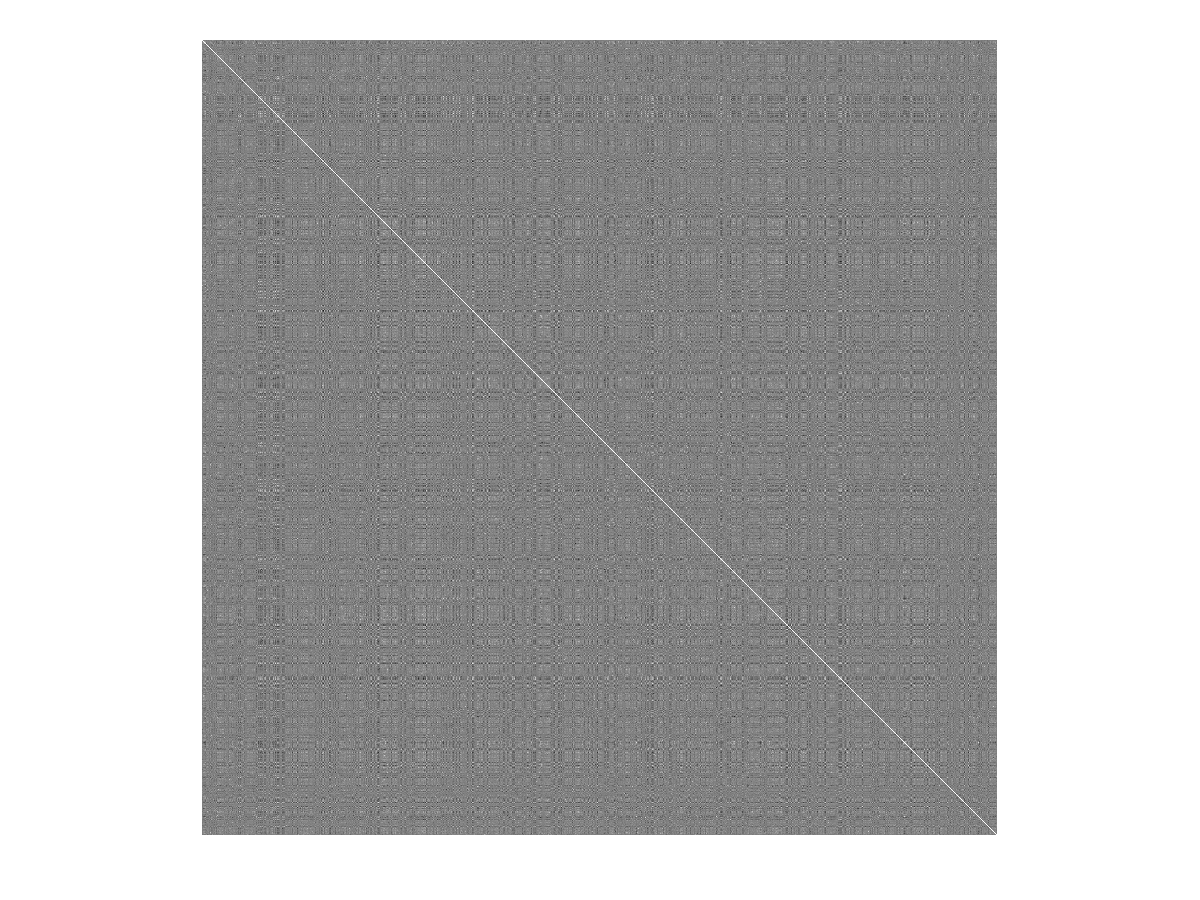
\includegraphics[scale=0.50]{figs/0.output.5sw.png}
\caption{A sample coffecient matrix: layer 1}
\end{figure}
The average abs coefficient value of each layer, however, is ascending(It's the only positive result I get).

%%%%%%%%%%%%%%%%%%%%%%%%%%%%%%%%%%%%%%%%%%%%%%%%%%%%%%%%%%%%%%%%%%%%%%%%%%%%%%%%%
\section{Experiment result}
Based on our intuition, we did some experiments. They are on 40-hour Chinese dataset.
\begin{table}[htb]
\begin{tabular}{|c|c|c|c|c|c|}
\hline
\hline
Wnumber & config(input$->$output) & feature & WER & CER & comment\\
\hline
& 512-512-512-512-512 & fbank & 37.57 & 31.46 &\\
\hline
& 512-512-512-1024-1024 & fbank & 36.35 & 30.34 & \textbf{strangly good, I need to run another to verify}\\
\hline
& 512-512-512-512-1024 & fbank & 37.08 & 30.08 & now running \\
\hline
& 1024-1024-512-512-512 & fbank & 37.08 & 31.00 & improved only a little, not good\\
\hline
& 1024-1024-1024-1024-1024 & fbank & 35.79 & 29.71 &\\
\hline
\hline
& 2048-2048-2048-2048-2048 & mfcc & 43.00 & 35.84 & \\
\hline
6760448 & 1024-1024-1024-1024-1024 & mfcc & 43.17 & 36.57 & \\
\hline
 & 1024-1024-512-512-512 & mfcc & 42.41 & 36.06 & ridiculous!\\
\hline
& 1224-1224-1224-1024-930 & mfcc & 43.10 & 36.42 & improved a little\\
\hline
& 512-512-512-512-512 & mfcc & 44.68 & 38.47 & \\
\hline
& 4096-1024-256 & mfcc & 43.50 & 37.23 & \\
\hline
6807168 & 4096-1024-512-128 & mfcc & 42.34 & 35.79  \\
\hline
\end{tabular}
\caption{Experiment result}
\end{table}

\section{concrete staticistic}
\begin{verbatim}
FIRST PASS:NO SMOOTH
average bin entropy using 2 bins for input.output.5sw is 0.99680
average bin entropy using 10 bins for input.output.5sw is 1.12812
average bin entropy using 100 bins for input.output.5sw is 3.69362
average parzen entropy for input.output.5sw is 1.78861
have 0 NaN for coe
average abs coefficient for input.output.5sw is 0.09499

average bin entropy using 2 bins for 0.output.5sw is 0.61915
average bin entropy using 10 bins for 0.output.5sw is 1.48369
average bin entropy using 100 bins for 0.output.5sw is 3.11048
average parzen entropy for 0.output.5sw is -7.02191
have 0 NaN for coe
average abs coefficient for 0.output.5sw is 0.00977

average bin entropy using 2 bins for 1.output.5sw is 0.47607
average bin entropy using 10 bins for 1.output.5sw is 1.52977
average bin entropy using 100 bins for 1.output.5sw is 3.77994
average parzen entropy for 1.output.5sw is -3.47713
have 0 NaN for coe
average abs coefficient for 1.output.5sw is 0.02989

average bin entropy using 2 bins for 2.output.5sw is 0.45816
average bin entropy using 10 bins for 2.output.5sw is 1.62125
average bin entropy using 100 bins for 2.output.5sw is 4.06034
average parzen entropy for 2.output.5sw is -2.43128
have 0 NaN for coe
average abs coefficient for 2.output.5sw is 0.03447

average bin entropy using 2 bins for 3.output.5sw is 0.52065
average bin entropy using 10 bins for 3.output.5sw is 1.87043
average bin entropy using 100 bins for 3.output.5sw is 4.58371
average parzen entropy for 3.output.5sw is -1.89372
have 0 NaN for coe
average abs coefficient for 3.output.5sw is 0.04152

average bin entropy using 2 bins for 4.output.5sw is 0.39158
average bin entropy using 10 bins for 4.output.5sw is 1.31739
average bin entropy using 100 bins for 4.output.5sw is 3.40673
average parzen entropy for 4.output.5sw is -3.03547
have 0 NaN for coe
average abs coefficient for 4.output.5sw is 0.03969

average bin entropy using 2 bins for before_softmax.output.1sw is 0.39306
average bin entropy using 10 bins for before_softmax.output.1sw is 1.45831
average bin entropy using 100 bins for before_softmax.output.1sw is 4.50276
average parzen entropy for before_softmax.output.1sw is 3.36435
have 0 NaN for coe
average abs coefficient for before_softmax.output.1sw is 0.00046



SECOND PASS:HTXSMOOTH
number 0 in sh is 0
average bin entropy using 10 bins for 0.output is 1.49398
Elapsed time is 48.578395 seconds.
calculating bin entropy seriously...
number 0 in sh is 0
average bin entropy using 100 bins for 0.output is 3.13192
Elapsed time is 66.820899 seconds.
calculating bin entropy seriously...
number 0 in sh is 0
average bin entropy using 1000 bins for 0.output is 5.18421
Elapsed time is 89.725121 seconds.
loading file 1.output...
calculating bin entropy seriously...
number 0 in sh is 0
average bin entropy using 10 bins for 1.output is 1.53160
Elapsed time is 74.975033 seconds.
calculating bin entropy seriously...
number 0 in sh is 0
average bin entropy using 100 bins for 1.output is 3.78013
Elapsed time is 97.759049 seconds.
calculating bin entropy seriously...
number 0 in sh is 0
average bin entropy using 1000 bins for 1.output is 6.65583
Elapsed time is 137.379478 seconds.
loading file 2.output...
calculating bin entropy seriously...
number 0 in sh is 0
average bin entropy using 10 bins for 2.output is 1.67506
Elapsed time is 68.782464 seconds.
calculating bin entropy seriously...
number 0 in sh is 0
average bin entropy using 100 bins for 2.output is 4.08831
Elapsed time is 107.783938 seconds.
calculating bin entropy seriously...
number 0 in sh is 0
average bin entropy using 1000 bins for 2.output is 7.07061
Elapsed time is 141.556137 seconds.
loading file 3.output...
calculating bin entropy seriously...
number 0 in sh is 0
average bin entropy using 10 bins for 3.output is 1.87505
Elapsed time is 72.851595 seconds.
calculating bin entropy seriously...
number 0 in sh is 0
average bin entropy using 100 bins for 3.output is 4.58967
Elapsed time is 98.607577 seconds.
calculating bin entropy seriously...
number 0 in sh is 0
average bin entropy using 1000 bins for 3.output is 7.75323
Elapsed time is 144.474092 seconds.
loading file 4.output...
calculating bin entropy seriously...
number 0 in sh is 0
average bin entropy using 10 bins for 4.output is 1.32256
Elapsed time is 66.106949 seconds.
calculating bin entropy seriously...
number 0 in sh is 0
average bin entropy using 100 bins for 4.output is 3.41288
Elapsed time is 91.673775 seconds.
calculating bin entropy seriously...
number 0 in sh is 0
average bin entropy using 1000 bins for 4.output is 6.26242
Elapsed time is 121.617199 seconds.
loading file before_softmax.output...
calculating bin entropy seriously...
number 0 in sh is 0
average bin entropy using 10 bins for before_softmax.output is 1.43235
Elapsed time is 101.336213 seconds.
calculating bin entropy seriously...
number 0 in sh is 0
average bin entropy using 100 bins for before_softmax.output is 4.43838
Elapsed time is 145.667090 seconds.
calculating bin entropy seriously...
number 0 in sh is 0
average bin entropy using 1000 bins for before_softmax.output is 7.75483
Elapsed time is 228.666910 seconds.
loading file input.output...
calculating bin entropy seriously...
number 0 in sh is 0
average bin entropy using 10 bins for input.output is 1.13593
Elapsed time is 36.487177 seconds.
calculating bin entropy seriously...
number 0 in sh is 0
average bin entropy using 100 bins for input.output is 3.59119
Elapsed time is 52.837555 seconds.
calculating bin entropy seriously...
number 0 in sh is 0
average bin entropy using 1000 bins for input.output is 7.07143
Elapsed time is 82.983234 seconds.
\end{verbatim}
\end{document}
